\documentclass[12pt]{article}
\usepackage[margin=2.5cm]{geometry}
\usepackage{enumerate}
\usepackage{amsfonts}
\usepackage{amsmath}
\usepackage{fancyhdr}
\usepackage{amsmath}
\usepackage{amssymb}
\usepackage{amsthm}
\usepackage{mdframed}
\usepackage{graphicx}
\usepackage{subcaption}
\usepackage{adjustbox}
\usepackage{listings}
\usepackage{xcolor}
\usepackage{booktabs}
\usepackage[utf]{kotex}
\usepackage{hyperref}

\definecolor{codegreen}{rgb}{0,0.6,0}
\definecolor{codegray}{rgb}{0.5,0.5,0.5}
\definecolor{codepurple}{rgb}{0.58,0,0.82}
\definecolor{backcolour}{rgb}{0.95,0.95,0.92}

\lstdefinestyle{mystyle}{
    backgroundcolor=\color{backcolour},
    commentstyle=\color{codegreen},
    keywordstyle=\color{magenta},
    numberstyle=\tiny\color{codegray},
    stringstyle=\color{codepurple},
    basicstyle=\ttfamily\footnotesize,
    breakatwhitespace=false,
    breaklines=true,
    captionpos=b,
    keepspaces=true,
    numbers=left,
    numbersep=5pt,
    showspaces=false,
    showstringspaces=false,
    showtabs=false,
    tabsize=1
}

\lstset{style=mystyle}

\pagestyle{fancy}
\renewcommand{\headrulewidth}{0.4pt}
\lhead{CSC 209}
\rhead{Review 5 Solution}

\begin{document}
\title{CSC 209 Review 5 Solution}
\maketitle

\bigskip

\section{Exercises}

\begin{enumerate}[1.]
    \item

    \bigskip

    \begin{enumerate}[a)]
        \item 14
        \item 34
        \item 4
        \item true
        \item false
    \end{enumerate}

    \underline{\textbf{Notes}}

    \begin{itemize}
        \item \textbf{Pointer Arithematic}

        \begin{itemize}
            \item Adding an integer to a pointer

            \bigskip

            \underline{\textbf{Example}}

            \begin{center}
            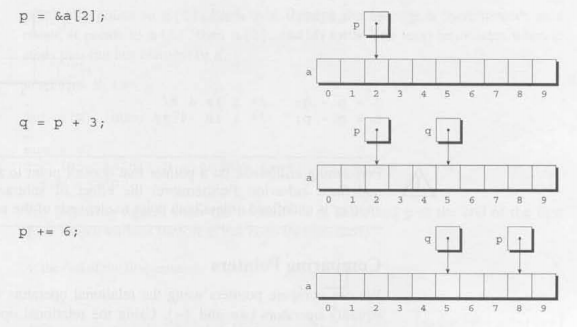
\includegraphics[width=\linewidth]{images/review_5_solution_1.png}
            \end{center}

            \bigskip

            \item Subtracting an integer from a pointer

            \bigskip

            \underline{\textbf{Example}}

            \begin{center}
            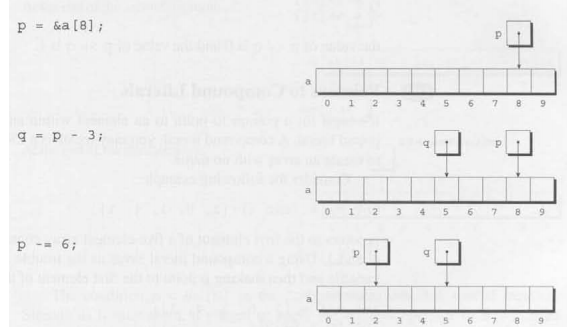
\includegraphics[width=\linewidth]{images/review_5_solution_2.png}
            \end{center}

            \bigskip

            \item Subtracting one pointer from another

            \bigskip

            \underline{\textbf{Example}}

            \begin{center}
            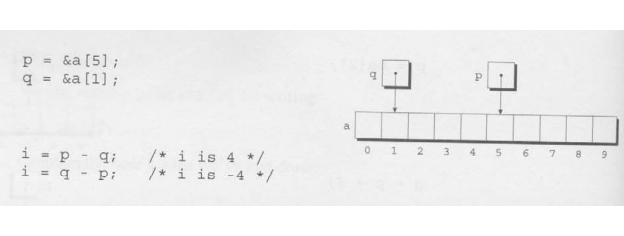
\includegraphics[width=\linewidth]{images/review_5_solution_3.png}
            \end{center}

        \end{itemize}

        \item \textbf{Comparing pointers}

        \begin{itemize}
            \item Can compare pointers using relational operators (i.e. $<,<=,>,>=$) and the equality operators (i.e. $==, !=$)
            \item Returns 1 if \texttt{true} and 0 if \texttt{false}

            \bigskip

            \underline{\textbf{Example}}

            \bigskip

            \texttt{p = \&a[5];}

            \texttt{q = \&a[1];}

            \bigskip

            \texttt{p $<=$ q} is 0 and \texttt{p $>=$ q} is 1


        \end{itemize}


    \end{itemize}

    \item

    \bigskip

    \texttt{low} and \texttt{high} are memory addresses.

    \bigskip

    So, \texttt{low $+$ high} is out of bound, and it could potentially point to an undesirable or wrong value.

    \bigskip

    To fix this, we subtract the from high value to the low value:

    \bigskip

    \begin{align}
        \texttt{middle} = \frac{\texttt{low $+$ high}}{2}
    \end{align}

    \item

    \bigskip

    I need to write the contents of an array \texttt{a} after the execution of
    statements outlined in problem sheet.

    \bigskip

    After execution, the array would have contents of $[10,9,8,7,6,5,4,3,2,1]$.

    \bigskip

    \underline{\textbf{Notes}}

    \begin{itemize}
        \item \textbf{Combining the * and ++ Operators}

        \begin{itemize}
            \item \texttt{*p++} or \texttt{*{p++}} $\to$ Value of expression is \texttt{*p} before increment; increment \texttt{p} later
            \item \texttt{(*p)++} $\to$ Value of expression is \texttt{*p} before increment; increment \texttt{*p} later
            \item \texttt{*++p} or \texttt{*(++p)} $\to$ Increment \texttt{p} first; value of expression is \texttt{*p} after increment
            \item \texttt{++*p} or \texttt{++(*p)} $\to$ Increment \texttt{*p} first; value of expression is \texttt{*p} after increment
        \end{itemize}

        \bigskip

        \underline{\textbf{Example}}

        \bigskip

        \texttt{a[i++] = j}

        \bigskip

        Means assign the value \texttt{j} to \texttt{a[i]} before increment

        \bigskip

        \underline{\textbf{Example 2}}

        \bigskip

        \begin{center}
        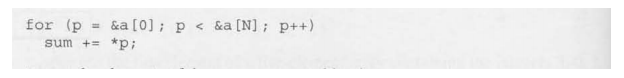
\includegraphics[width=\linewidth]{images/review_5_solution_4.png}
        \end{center}

        Is the same as

        \begin{center}
        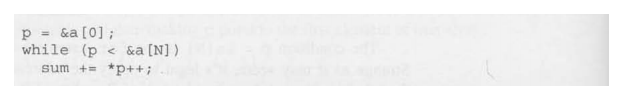
\includegraphics[width=\linewidth]{images/review_5_solution_5.png}
        \end{center}
    \end{itemize}

    \item

    I need to re-write prototype \texttt{make\_empty}, \texttt{is\_empty} and \texttt{is\_full}
    of the following code to use the pointer variable \texttt{top\_ptr} instead of the integer
    variable \texttt{top}.

    \bigskip

\begin{lstlisting}[language=c]
    #include <stdbool.h>

    #define STACK_SIZE 100

    /*external variables*/
    int contents[STACK_SIZE]
    int top = 0;

    void make_empty(void) {
        top = 0;
    }

    bool is_empty(void) {
        return top == 0;
    }

    bool is_full(void) {
        return top == STACK_SIZE;
    }
\end{lstlisting}

    \bigskip

    And after re-write using \texttt{top\_ptr} instead of \texttt{top} have:


\begin{lstlisting}[language=c]
    #include <stdbool.h>

    #define STACK_SIZE 100

    /*external variables*/
    int contents[STACK_SIZE]
    int *top_ptr = &contents[0];

    void make_empty(void) {
        top_ptr = &contents[0];
    }

    bool is_empty(void) {
        return top_ptr == &contents[0];
    }

    bool is_full(void) {
        return top_ptr == &contents[STACK_SIZE-1];
    }
\end{lstlisting}

    \item

    First, I need to identify which of the following expressions are illegal
    because of mismatched types.

    \bigskip

    \begin{enumerate}[a)]
        \item \texttt{p $==$ a[0]}
        \item \texttt{p $==$ \&a[0]}
        \item \texttt{*p $==$ a[0]}
        \item \texttt{p[0] == a[0]}
    \end{enumerate}

    \bigskip

    Here, only \texttt{a)} is illegal.

    \bigskip

    Second, I need to write which of the remaining expressions are true.

    \bigskip

    Here, the expressions that return true are \texttt{b)}, \texttt{c)} and \texttt{d)}.

    \bigskip

    \underline{\textbf{Notes}}

    \begin{itemize}
        \item \texttt{*(a+i)} is equal to \texttt{a[i]}
        \item \texttt{*p} and \texttt{a[]} are the same given \texttt{p $==$ a}
        \item \textbf{Using an Array Name as a Pointer}

        \begin{itemize}
            \item The name of an array can be used as a pointer to the first element in the array.

            \bigskip

            \underline{\textbf{Example}}

            \bigskip

            \texttt{int a[10];}

            \bigskip

            \texttt{*a = 7; /* stores 7 in a[0] */}

            \bigskip

            \texttt{*(a+1) = 12; /* stores 7 in a[1] */}

            \bigskip

            \underline{\textbf{Example 2}}

            \bigskip

            \begin{center}
            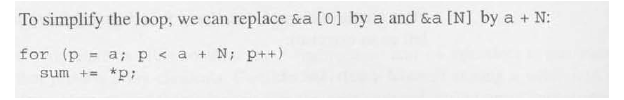
\includegraphics[width=\linewidth]{images/review_5_solution_6.png}
            \end{center}

        \end{itemize}
    \end{itemize}

    \item

    I need to re-write the following to use pointer arithematic instead
    of array subscripting, and I need to make as few change as possible.

    \bigskip

\begin{lstlisting}[language=c]
    int sum_array(cost int a[], int n) {
        int i, sum;

        sum = 0;

        for (i = 0; i < n; i++)
            sum += a[i];
        return sum;
    }
\end{lstlisting}

    \bigskip

    After making changes to above code to use pointer arithematic, we have

\begin{lstlisting}[language=c]
    int sum_array(cost int a[], int n) {
        int i, sum;

        sum = 0;

        for (i = 0; i < n; i++)
            sum += *(a+i);
        return sum;
    }
\end{lstlisting}

    \item

    I need to write the following using pointer arithematic so it finds an element
    in \texttt{a} that matches to value \texttt{key}. I need to return
    true if there is a match.

    \bigskip

    \texttt{bool search(const int a[], int n, int key);}

    \bigskip

    And the solution is:

\begin{lstlisting}[language=c]
    bool search(cost int a[], int n, int key) {

        for (int i = 0; i < n; i++) {
            if (*(a+i) == key) {
                return true
            }
        }

        return false;
    }
\end{lstlisting}

    \item

    Here, I need to re-write the following function to use pointer arithmetic
    instead of array subscripting.

    \bigskip

\begin{lstlisting}[language=c]
    void store_zeros(cost int a[], int n) {
        int i;

        for (i = 0; i < n; i++) {
            a[i] = 0;
        }
    }
\end{lstlisting}

    \bigskip

    After re-writing above code, we have

\begin{lstlisting}[language=c]
    void store_zeros(cost int a[], int n) {
        int *p;

        for (p = a; p < a + n; p++) {
            *p = 0;
        }
    }
\end{lstlisting}

    \item

    Here, I need to write the function

    \bigskip

    \texttt{double inner\_product(const double *a, const double *b, int n)}

    \bigskip

    using pointer arithmetic such that it returns \texttt{a[0] * b[0] + a[1] *
    b[1] + a[2] * b[2] + ... + a[n-1] * b[n-1]}.

    \bigskip

    The solution is provided below

    \bigskip

\begin{lstlisting}[language=c]
    double inner_product(const double *a, const double *b, int n) {
        double sum = 0, p*;

        p = a;

        while (p < a + n) {
            sum += *a * *b;

            a++;
            b++;
            p++;
        }

        return sum;
    }
\end{lstlisting}

    \bigskip

    \begin{mdframed}
        \underline{\textbf{Correct Solution}}

        \bigskip

\begin{lstlisting}[language=c]
double inner_product(const double *a, const double *b, int n) {
    double sum = 0, *p;

    p = a;

    while (p++ < a + n) {
        sum += *a++ * *b++;
    }

    return sum;
}
\end{lstlisting}

    \end{mdframed}

    \item

    Here, I need to rewrite the function \texttt{find\_middle} so that it uses
    pointer arithmetic - not subscripting - to visit any element.

    \bigskip

    The solution to this exercise is provided below.

    \bigskip

\begin{lstlisting}[language=c]
    int *find_middle(int a[], int n) {
        return a + (n/2)
    }
\end{lstlisting}

    \item

    Here I need to modify the function \texttt{find\_largest} function so that it
    uses pointer arithmetic - not subscripting - to visit array elements

    \bigskip

\begin{lstlisting}[language=c]
    int *find_largest(int a[], int n) {
        int *p, *max;

        max = a;

        for (p = a; p < a + n; p++){
            if (*p > *max) {
                max = p;
            }
        }

        return *max;
    }
\end{lstlisting}

    \item

    I need to write the function

    \bigskip

    \texttt{void find\_two\_largest(const int *a, int n, int *largest, int *second\_largest)}

    \bigskip

    using pointer arithmetic.

    \bigskip

    The solution to this exercise is:

    \bigskip


\begin{lstlisting}[language=c]
    #include <stdbool.h> // bool
    #include <limits.h>  // INT_MIN

    bool is_largest(int current_max, int val);

    void find_two_largest (int a[], int n, int *largest, int* second_largest) {
        int current_max = INT_MIN;
        int current_second_max = INT_MIN;

        for (int i = 0; i < n; i++) {
            if (is_largest(current_max, a[i])) {
                current_second_max = current_max;
                current_max = *(a + i);
            }
        }

        *largest = current_max;
        *second_largest = current_second_max;
    }

    bool is_largest(int current_max, int val) {
        if (val > current_max) {
            return true;
        }

        return false;
    }
\end{lstlisting}

    \bigskip

    \begin{mdframed}

    \underline{\textbf{Correct Solution:}}

    \bigskip

\begin{lstlisting}[language=c]
    void find_two_largest(const int *a, int n, int *largest, int *second_largest) {

        const int *p = a;
        *largest = *second_largest = *a;

        while (p++ < a + n) {
            if (*p > *largest) {
                *second_largest = *largest;
                *largest = *p;
            } else if (*p > *second_largest)
                *second_largest = *p;
        }
    }
\end{lstlisting}

    \end{mdframed}

    \item

    I need to rewrite the following program such that it uses a single pointer through
    the array one element at a time.

    \bigskip

\begin{lstlisting}[language=c]
    #define N 10

    double ident[N][N];
    int row, col;

    for (row = 0; row < N; row++) {
        for (col = 0; col < N; col++) {
            if (row == col) {
                ident[row][col] = 1.0;
            } else {
                ident[row][col] = 0.0;
            }
        }
    }
\end{lstlisting}

    \bigskip

    The solution to this exercise is:

    \bigskip

\begin{lstlisting}[language=c]
    #include <stdio.h>
    #include <stdbool.h>

    #define N 10

    bool is_row_eq_col(int i, int n);

    int main() {

        int i = 0;

        double ident[N][N], *p;


        for (p = &ident[0][0]; p < &ident[N-1][N-1]; p++) {
            if (is_row_eq_col(i, N)) {
                *p = 1.0;
            } else {
                *p = 0.0;
            }
            i++;
        }


        return 0;
    }

    bool is_row_eq_col(int i, int n) {
        if (i % (n+1) != 0) {
            return false;
        }

        return true;
    }
\end{lstlisting}

    \bigskip

    \underline{\textbf{Notes}}

    \begin{itemize}
        \item Learned that the memory address of each row in two dimensional array are placed
        right next to each other
    \end{itemize}


    \item

    I need to write a statement that uses the \texttt{search} function from Exercise 7
    to search the entire \texttt{temperatures} array for thevalue 32.

    \bigskip

    The solution to this problem is:

    \bigskip

\begin{lstlisting}[language=c]
    int row = 0;

    for (int row = 0; row < 7; row++) {
        if (search(temperatures[row], 24, 32)) {
            return true
        }
    }

    return false;

\end{lstlisting}

    \item

    Create a loop that prints all temperature readings in row \texttt{i} of the
    following array using a pointer to visit each element of the row.

    \bigskip

    \texttt{inte temperatures[7][24]}

    \bigskip

    The solution to this problem is:

    \bigskip

\begin{lstlisting}[language=c]
    int *p;

    for (p = &a[i]; p < &a[i] + 24; p++) {
        printf("%d", *p);
    }

\end{lstlisting}

    \bigskip

    \begin{mdframed}
    \underline{\textbf{Correct Solution:}}

\begin{lstlisting}[language=c]
    int *p;

    for (p = &temperatures[i]; p < &temperatures[i] + 24; p++) {
        printf("%d", *p);
    }

\end{lstlisting}

    \end{mdframed}

    \item

    I need to write a loop that prints the highest temperature in the \texttt{temperatures}
    array for each day of the week using \texttt{find\_largest} function.

    \bigskip

    The solution to this problem is:

    \bigskip

\begin{lstlisting}[language=c]
    int *p, *val;

    for (p = &temperatures[i]; p < &temperatures[i] + 24; p++) {
        val = find_largest(p, 24);
        printf("%d\n", *val);
    }

\end{lstlisting}

    \item

    I need to rewrite the following function to use pointer arithmetic
    and single loop, instead of array subscripting.

    \bigskip

\begin{lstlisting}[language=c]
    int sum_two_dimensional_array(const int a[][LEN], int n) {
        int i, j, sum = 0;

        for (i = 0; i < n; i++) {
            for (j = 0; j < LEN; j++) {
                sum += a[i][j];
            }
        }

        return sum;
    }

\end{lstlisting}

    \bigskip

    The solution to this problem is:

    \bigskip


    \begin{lstlisting}[language=c]
        int sum_two_dimensional_array(const int a[][LEN], int n) {
            int *p, sum = 0;

            for (p = &a[0][0]; p < &a[n-1][LEN-1]; p++) {
                sum += *p;
            }

            return sum;
        }
    \end{lstlisting}

    \item

    I need to rewrite the \texttt{evaluation\_position} function described in
    exercise 13 of chapter 9 using pointer arithmatic and single loop.

    \bigskip

    The solution to this problem is:

\begin{lstlisting}[language=c]
    int evaluate_position(char board[8][8]) {

        int white = 0, black = 0;
        char *p;

        for (p = &board[0][0]; p < &board[7][7]; p++) {
            switch(*p) {
                case 'Q':
                    white += 9;
                    break;
                case 'q':
                    black += 9;
                    break;
                case 'R':
                    white += 5;
                    break;
                case 'r':
                    black += 5;
                    break;
                case 'B':
                    white += 3;
                    break;
                case 'b':
                    black += 3;
                    break;
                case 'N':
                    white += 3;
                    break;
                case 'n':
                    black += 3;
                    break;
                case 'P':
                    white++;
                    break;
                case 'p':
                    black++;
                    break;
                default:
                    break;
            }
        }

        return white - black;
    }
\end{lstlisting}

    \bigskip

    \underline{\textbf{References}}

    \begin{enumerate}[1)]
        \item Githib (William Gherman), c-solutions (Chapter 9 Exercise 13), \href{https://github.com/williamgherman/c-solutions/tree/master/09/exercises/13}{link}
    \end{enumerate}


\section{Programming Projects}

\begin{enumerate}[1.]
    \item

    \begin{enumerate}[a)]
        \item

        I need to write a program that reads a message, then prints the reversal of the message.

        \bigskip

        The additional requirement for this program are:

        \begin{itemize}
            \item Read the message one character at a time using \texttt{getchar}
            \item Read characters should be stored in an array
            \item Read should be stopped when the array is full or the character read is `\texttt{$\backslash$n}'
        \end{itemize}

        \bigskip

        The solution to this problem is:

        \bigskip

\begin{lstlisting}[language=c]
    #include <stdio.h>

    #define SIZE 10

    int main(void) {

        char array[SIZE], c, temp;
        int i = 0, n;

        printf("Enter a message: ");

        // fill array
        do {
            c = getchar();

            if (c == '\n') {
                break;
            }

            array[i] = c;
            i++;
        } while (i < SIZE);

        n = i;

        // reverse characters in array

        for (int j = 0; j < (n - j); j++) {
            temp = array[j];
            array[j] = array[n - (1 + j)];
            array[n - (1 + j)] = temp;
        }

        printf("Reversal is: ");

        for (int j = 0; j < n; j++) {
            printf("%c", array[j]);
        }

        return 0;
    }
\end{lstlisting}

        \item

\begin{lstlisting}[language=c]
    #include <stdio.h>

    #define SIZE 10

    int main(void) {

        char array[SIZE], c, temp, *p;
        int i = 0, n;

        p = &array[0];

        printf("Enter a message: ");

        // fill array
        do {
            c = getchar();

            if (c == '\n') {
                break;
            }

            *p++ = c;
            i++;
        } while (p < array + SIZE);

        n = i;

        // reverse characters in array
        char *q = &array[0], *r = &array[n-1];

        while (q < r) {
            temp = *q;
            *q++ = *r;
            *r-- = temp;
        }

        printf("Reversal is: ");

        for (p = &array[0]; p < array + n; p++) {
            printf("%c", *p);
        }

        return 0;
    }
\end{lstlisting}

    \end{enumerate}

    \item

    \begin{enumerate}[a)]
        \item

        I need write a program that reads a message and checks if it's a palindrome.

        \bigskip

        The solution to this problem is:

        \bigskip

\begin{lstlisting}[language=c]
    #include <stdio.h>
    #include <stdbool.h>
    #include <ctype.h>

    #define SIZE 100

    bool is_palindrome(char array[], int n);

    int main(void) {
        char array[SIZE], c;
        int n = 0;

        // Read characters
        // Put characters into array
        printf("Enter a message: ");

        do {
            c = getchar();

            if (c == '\n') {
                break;
            }

            if (!isalpha(c)) {
                continue;
            }

            array[n] = tolower(c);
            n++;
        } while (n < SIZE);

        // Check if characters in array is palindrome
        if (is_palindrome(array, n)) {
            printf("Palindrome");
        } else {
            printf("Not a Palindrome");
        }

        return 0;
    }

    bool is_palindrome(char array[], int n) {
        char temp;

        for (int i = 0; i < (n - i); i++) {
            if (array[i] != array[n - (1 + i)]) {
                return false;
            }
        }

        return true;
    }
\end{lstlisting}

    \end{enumerate}
\end{enumerate}

\end{enumerate}

\end{document}